\section{Statistical Analysis}
\label{sec:statistical_analysis}

\todo[inline]{Fit, limits, treatment of systematics in fit}

Why binned likelihood (and not unbinned)?

Directly fit MVA score.


\subsection{Binning Algorithm}
\label{sec:binning_alg}

The signal sensitivity of a binned maximum likelihood fit of
MVA scores depends strongly on the choice of binning used for the
discriminant. The purity of signal increases with increasing MVA
score, with most signal (background) being concentrated at the highest
(lowest) MVA scores. For optimal expected signal sensitivity, the
binning has to be chosen such that regions in MVA score with low
signal-to-background ratio are separated from regions with high
signal-to-background ratio.

In this analysis an iterative re-binning algorithm is used to provide
the binning of the discriminants for the likelihood fits. The aim of
the algorithm is to provide good expected signal sensitivity while
ensuring that the background model obeys predefined constraints on the
statistical uncertainty and expected number of events in each bin. The
constraints are intended to stabilise the likelihood fits and ensure
reasonable validity of the asymptotic approximations used for the
sampling distributions of test statistics used in the statistical
analysis. The algorithm was previously used
in~\cite{HIGG-2016-16-witherratum} and is continued to be used in the
\hadhad channel of this search. A different algorithm, while
conceptually similar, is used in the \lephad channel and is
detailed~\cite{ATLAS-CONF-2021-030}.

The re-binning algorithm is provided with MVA score histograms with
fine, equidistant binning ($N_\text{bins} = 1000$) for the signal and
total background expectation. It proceeds by iteratively merging bins,
starting from the most-signal like MVA score bins, until the bin
fulfills a set of requirements:
\begin{enumerate}

\item The relative statistical uncertainty of the background in the
  bin must be smaller
  than~\mbox{$\SI{50}{\percent} \cdot f_\text{s} + \SI{1}{\percent}$},
  where $f_\text{s}$ is the fraction of signal events entering the bin
  relative to the expected number of signal events in the signal
  region. This requirement limits the statistical uncertainty on the
  background in the most signal-like bins after re-binning to be in
  the range of \SIrange{10}{20}{\percent}.

\item The expected number of background events in the bin must be
  larger than 5.

\end{enumerate}
When a bin fulfilling all requirements is found, the process is
repeated starting from the next un-merged bin. The algorithm
terminates with a final bin at low MVA score. If the final bin does
not fulfil the criteria, it is merged with the preceeding (already
merged) bin.

% The algorithm provides a binning that improves the analysis
% sensitivity while fulfilling criteria on the background model:
% I.e. that it has reasonable statistical precision, and that one
% expects at least 5 events so that asymptotic approximations of the
% test statistics can be used.


% Motivation of terms:
% 1\% have some bins in background dominated region
% signal fraction weighted 50\% to have relatively fine bins in the most signal-like regions

The size of bins resulting from the re-binning procedure can vary by
multiple orders of magnitude. For better visualisation of the bin
contents, the MVA scores are displayed as equidistant bins.

\todo[inline]{Visualise the rebinning somehow?}

\subsection{Results}

\begin{figure}[htbp]
  \centering

  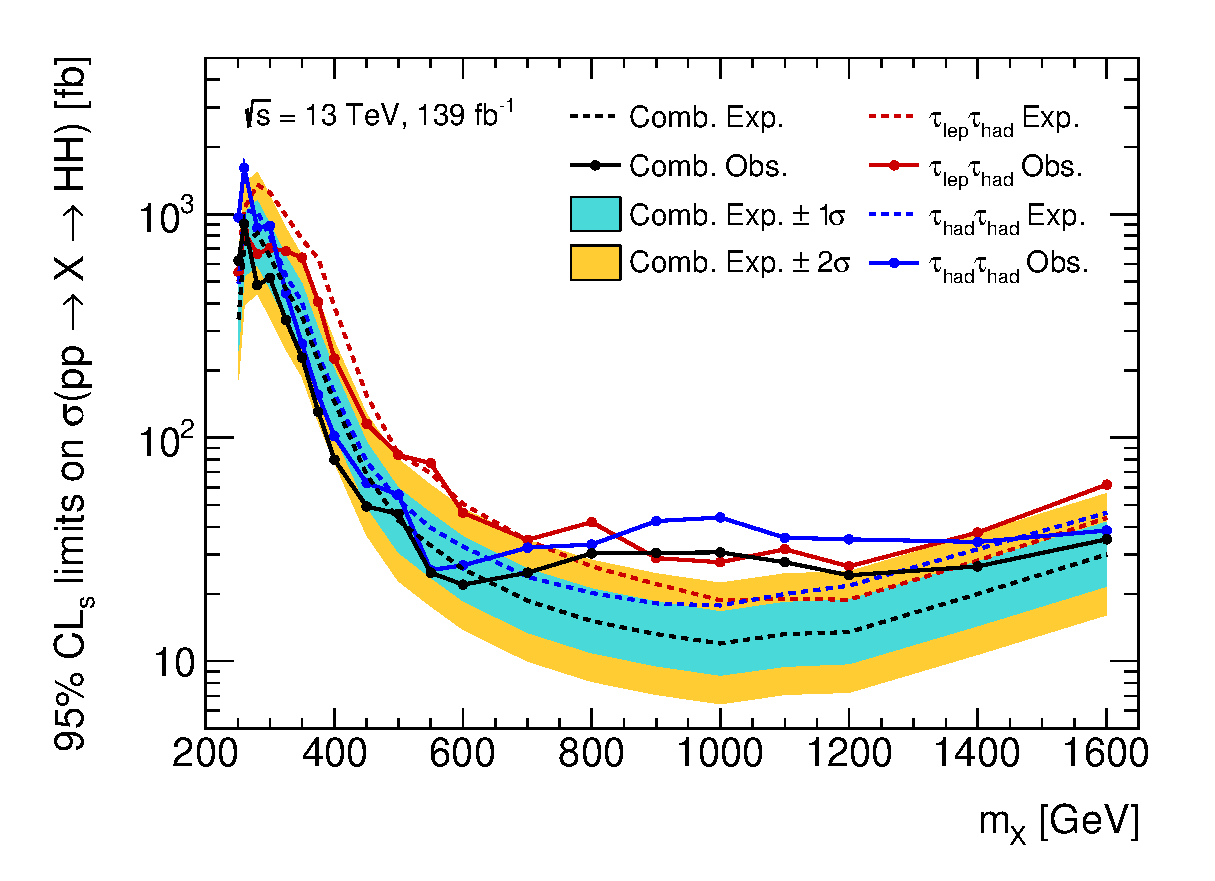
\includegraphics[width=0.65\textwidth]{results/resonant_comb_upper_limits}

  \caption{Upper limits for the resonant search}
  \label{fig:res_upper_limits}
\end{figure}

\begin{figure}[htbp]
  \centering

  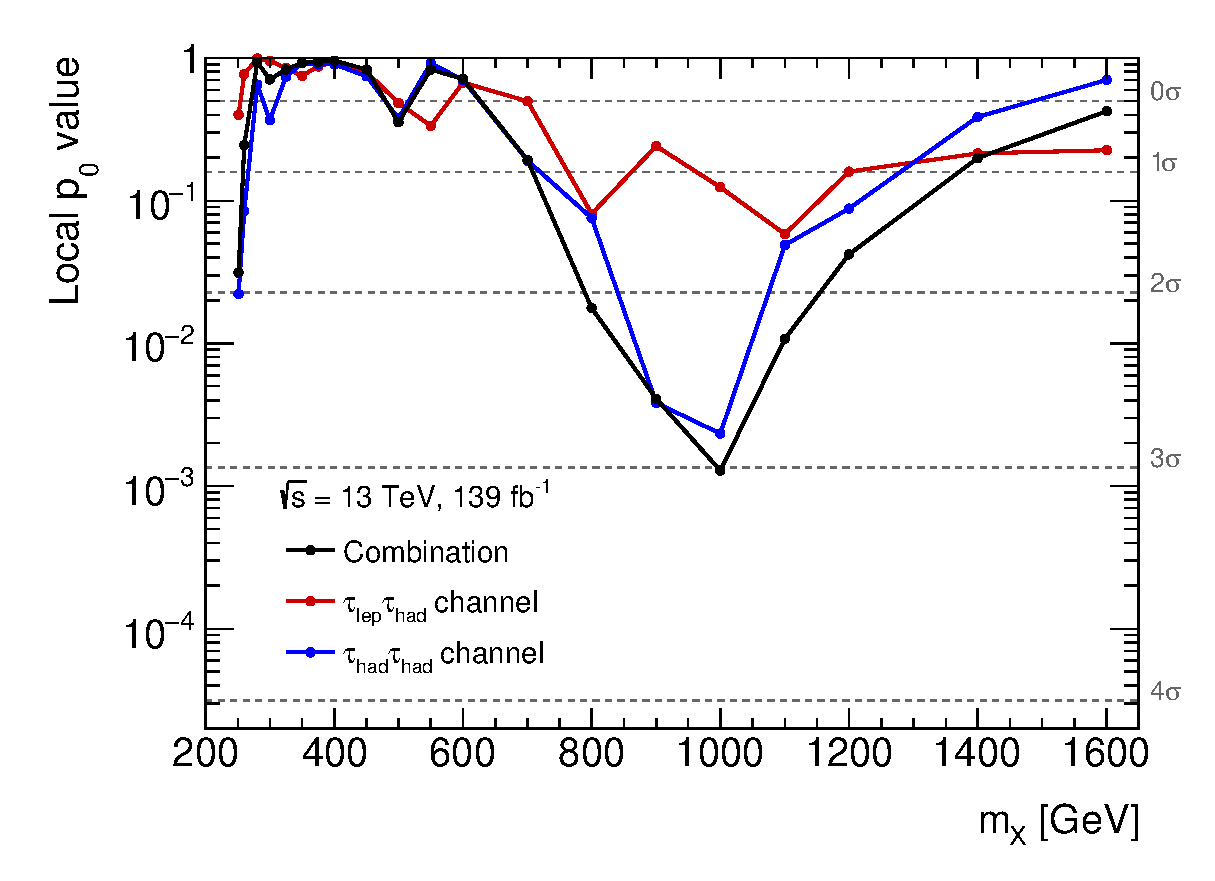
\includegraphics[width=0.65\textwidth]{results/resonant_comb_pvalues}

  \caption{Local pvalue scan}
  \label{fig:local_pvalues}
\end{figure}

\subsection{Discussion}



\begin{table}[htbp]
  \centering

  \begin{tabular}{lSS}
    \toprule
    & \multicolumn{2}{c}{Expected number of events} \\
    Process & {Last two bins} & {Last bin} \\
    \midrule
    \ZHF & 6.9 & \\
    Single Higgs boson & 6.9 & \\
    \ttbar & 4.6 & \\
    \jettotauhadvis (\ttbar) & 3.4 & \\
    \jettotauhadvis (multi-jet) & 2.2 & \\
    Other & 1.8 & \\
    \midrule
    Total background & & \\
    \midrule
    SM \HH (gluon fusion) & & \\
    SM \HH (VBF) & & \\
    \bottomrule
  \end{tabular}

  \caption{Table of expected yields. The uncertainties are from
    statistical sources only.}
  \todo[inline]{Post-fit yields}
\end{table}


%%% Local Variables:
%%% mode: latex
%%% TeX-master: "../../phd_thesis"
%%% End:
